\newpage
\section{Vector Load-store Unit}
\label{sec:memory}

\begin{figure}[h]
  \centering
  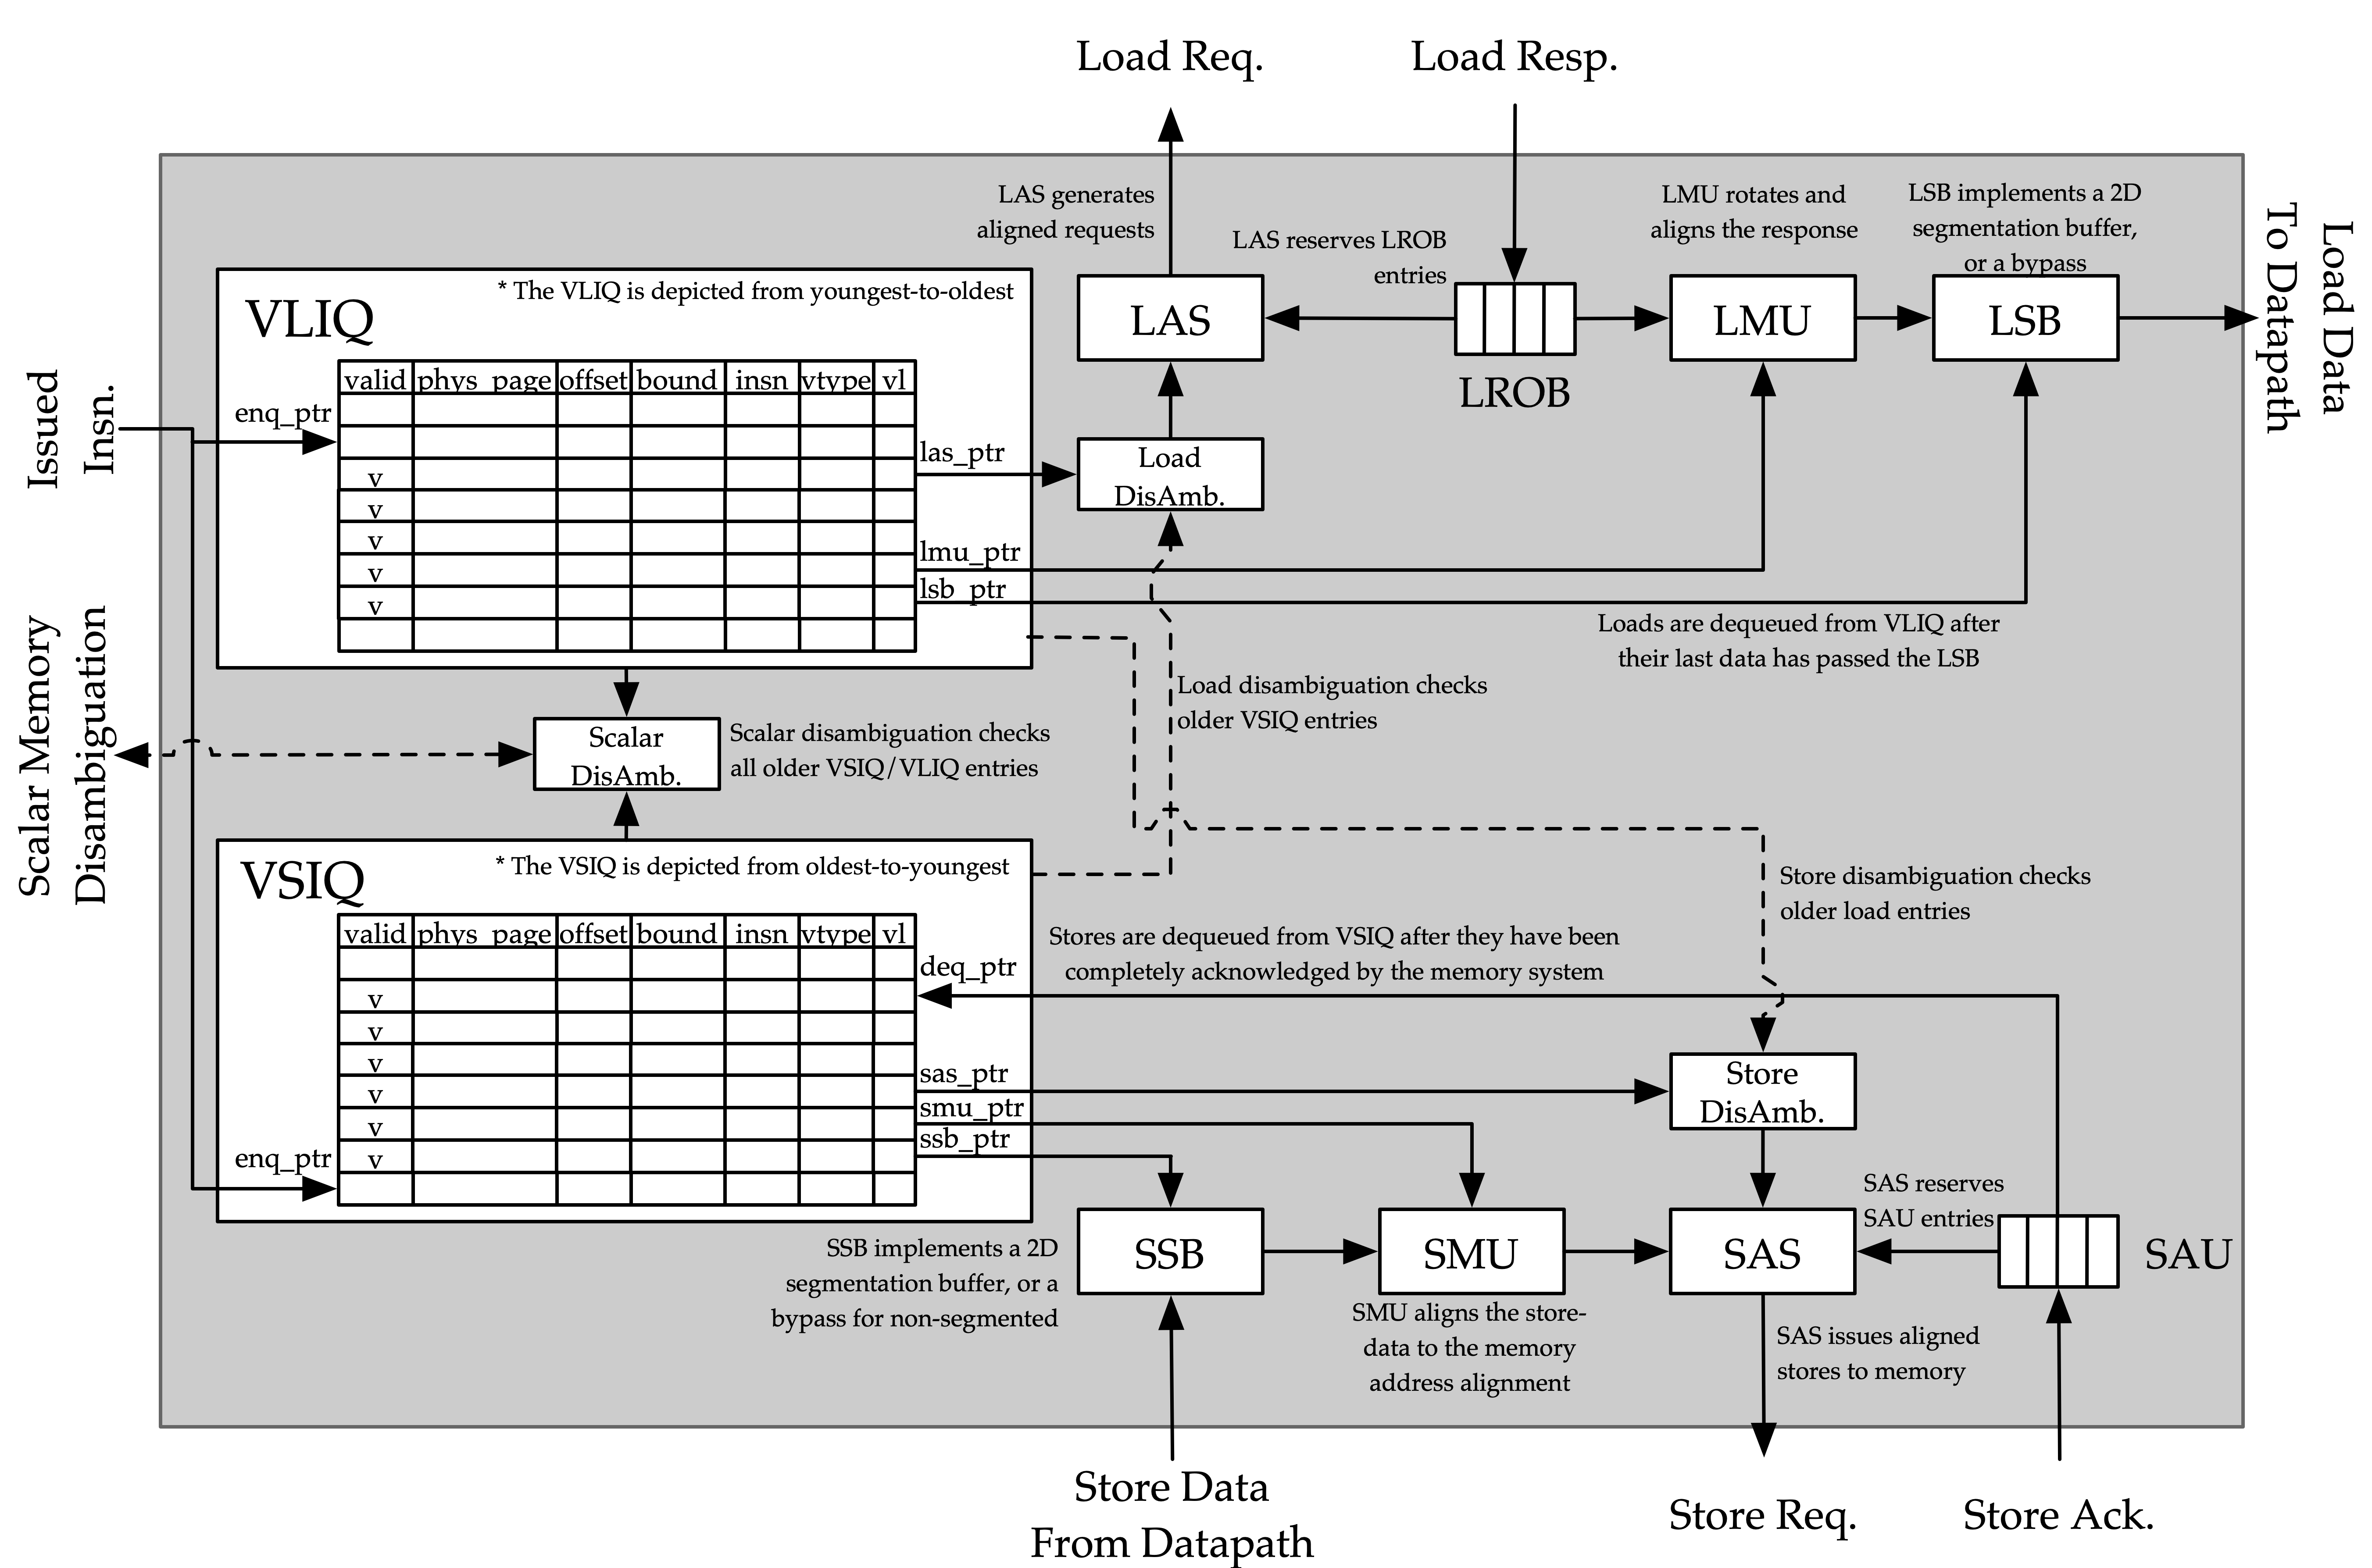
\includegraphics[width=\linewidth]{lsu.png}
  \caption{Vector Load-Store Unit Diagram}
  \label{fig:lsu}
\end{figure}

The Vector Load-Store Unit (VLSU) contains independent paths for loads and stores and is decoupled from the vector datapath (VU).
The load path performs load address generation and reformats load responses into load writebacks.
The store path performs store address generation and reformats vector register data into store requests.
Each path is designed to saturate a block memory interface that is \texttt{DLEN} bits wide.

The load and store paths are each designed as an in-order pipeline of units with latency-insensitive interfaces.
The control signals for each unit are driven by pointers into the load/store instruction queues (VLIQ/VSIQ).
Since independent pointers for each unit are maintained, each unit can operate on the same, or different instructions within the queues.
After an instruction has finished execution through the load or store path, its entry in the instruction queue is freed.

The load path consists of the following stages:

\begin{itemize}
\item Load Address Sequencer (LAS)
\item Load Reordering Buffer (LROB)
\item Load Response Merger (LMU)
\item Load Segment Buffer (LSB)
\end{itemize}
 
The store path consists of the following stages:

\begin{itemize}
\item Store Segment Buffer (SSB)
\item Store Data Merger (SMU)
\item Store Address Sequencer (SAS)
\item Store Acknowledgement Unit (SAU)
\end{itemize}
 
The store path is very similar to the reverse of the load path.
Notably, the SAS is identical to the LAS, while the SMU is identical to the LMU.

The VLSU additionally contains a separate address sequencer for accessing a specialized memory region for high throughput scatter and gather - the Scatter-Gather Address Sequencer (SGAS).
Indexed loads and stores that access a physical region managed by the scatter-gather memory use the SGAS for address sequencing, instead of the LAS or SAS, respectively.

\subsection{Memory System}

Saturn is designed for integration into a memory system that maintains coherence between VLSU accesses and scalar accesses into a scalar L1.
The VLSU exposes a generic load/store decoupled request and response interface.
This is typically converted into a coherent TileLink interface within either Rocket or Shuttle, but could be extended in the future to expose an incoherent AXI port instead.

\begin{figure}[h]
  \centering
  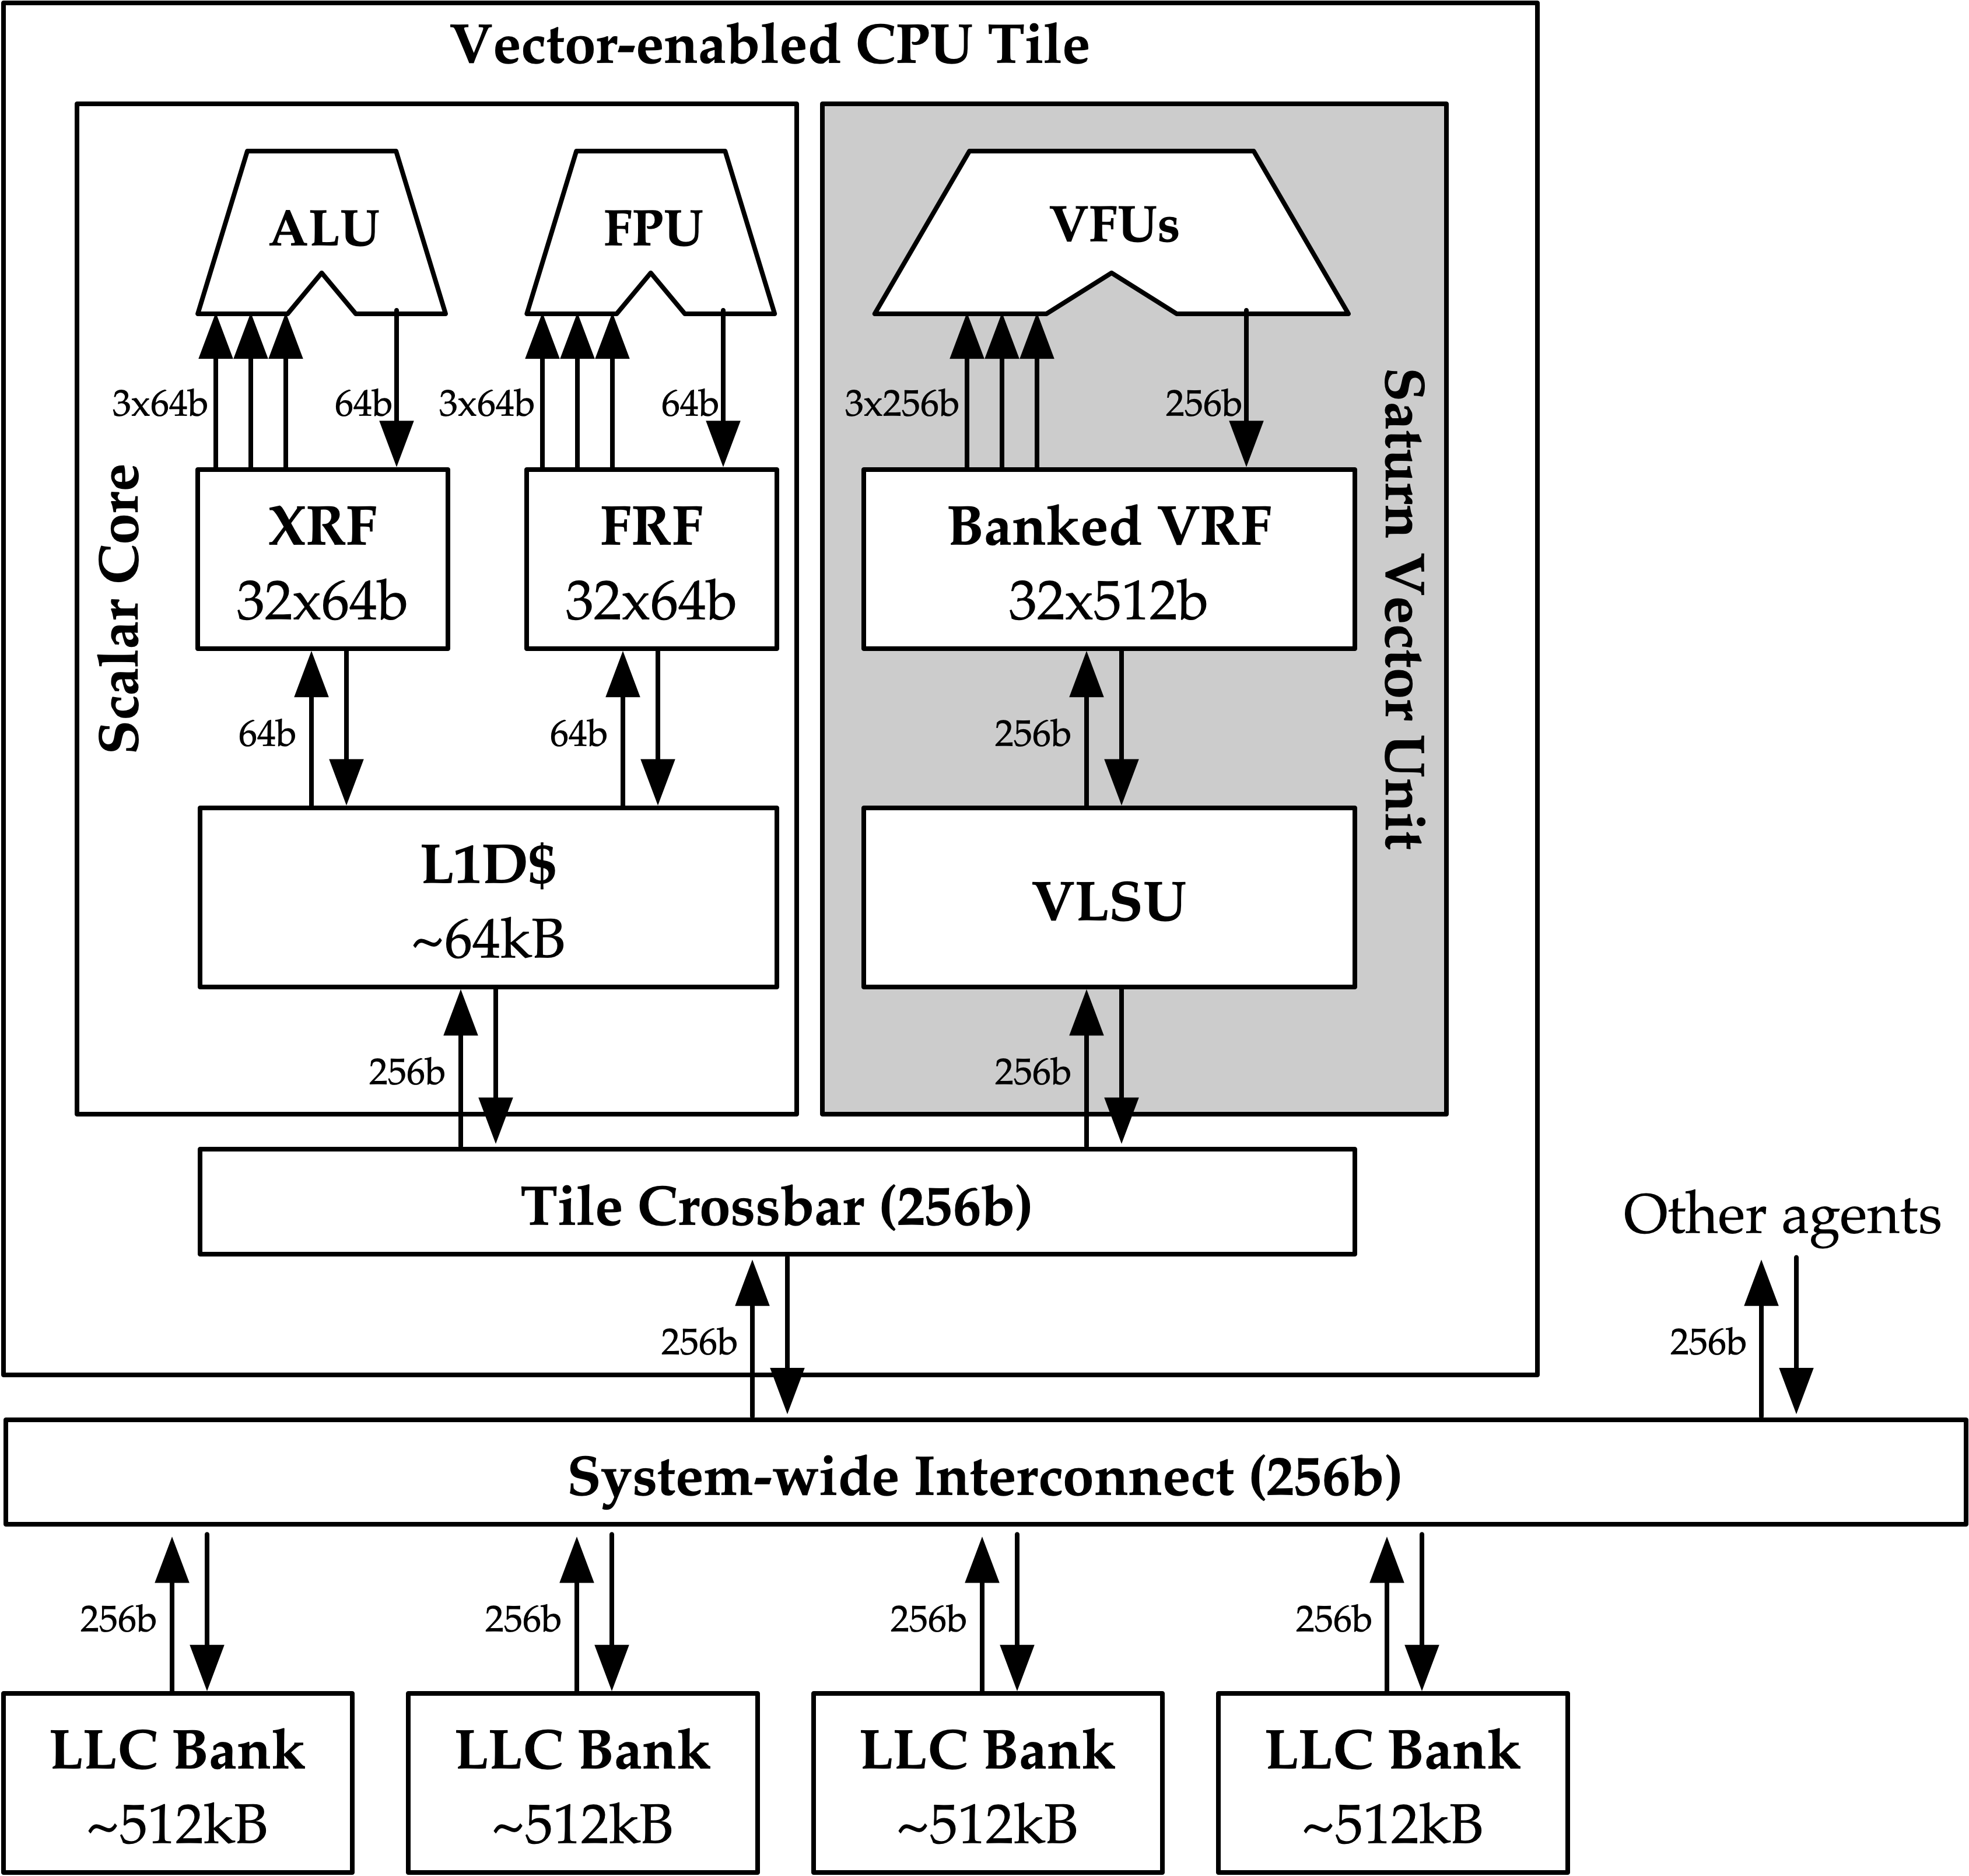
\includegraphics[scale=0.5]{memdefault.png}
  \caption{Example default configuration of the Saturn memory system}
  \label{fig:mem-default}
\end{figure}

One approach for the VLSU would be to direct all vector memory accesses into the scalar L1.
While simple, such a design would induce frequent structural hazards and require a specialized host core with a specialized L1 data cache.

While the Saturn integration with Rocket does support this approach, the standard and preferred mechanism is to provide a vector-specific memory port that bypasses the L1 and accesses coherent backing memory.
Figure \ref{fig:mem-default} depicts such a memory system.


\begin{figure}[h]
  \centering
  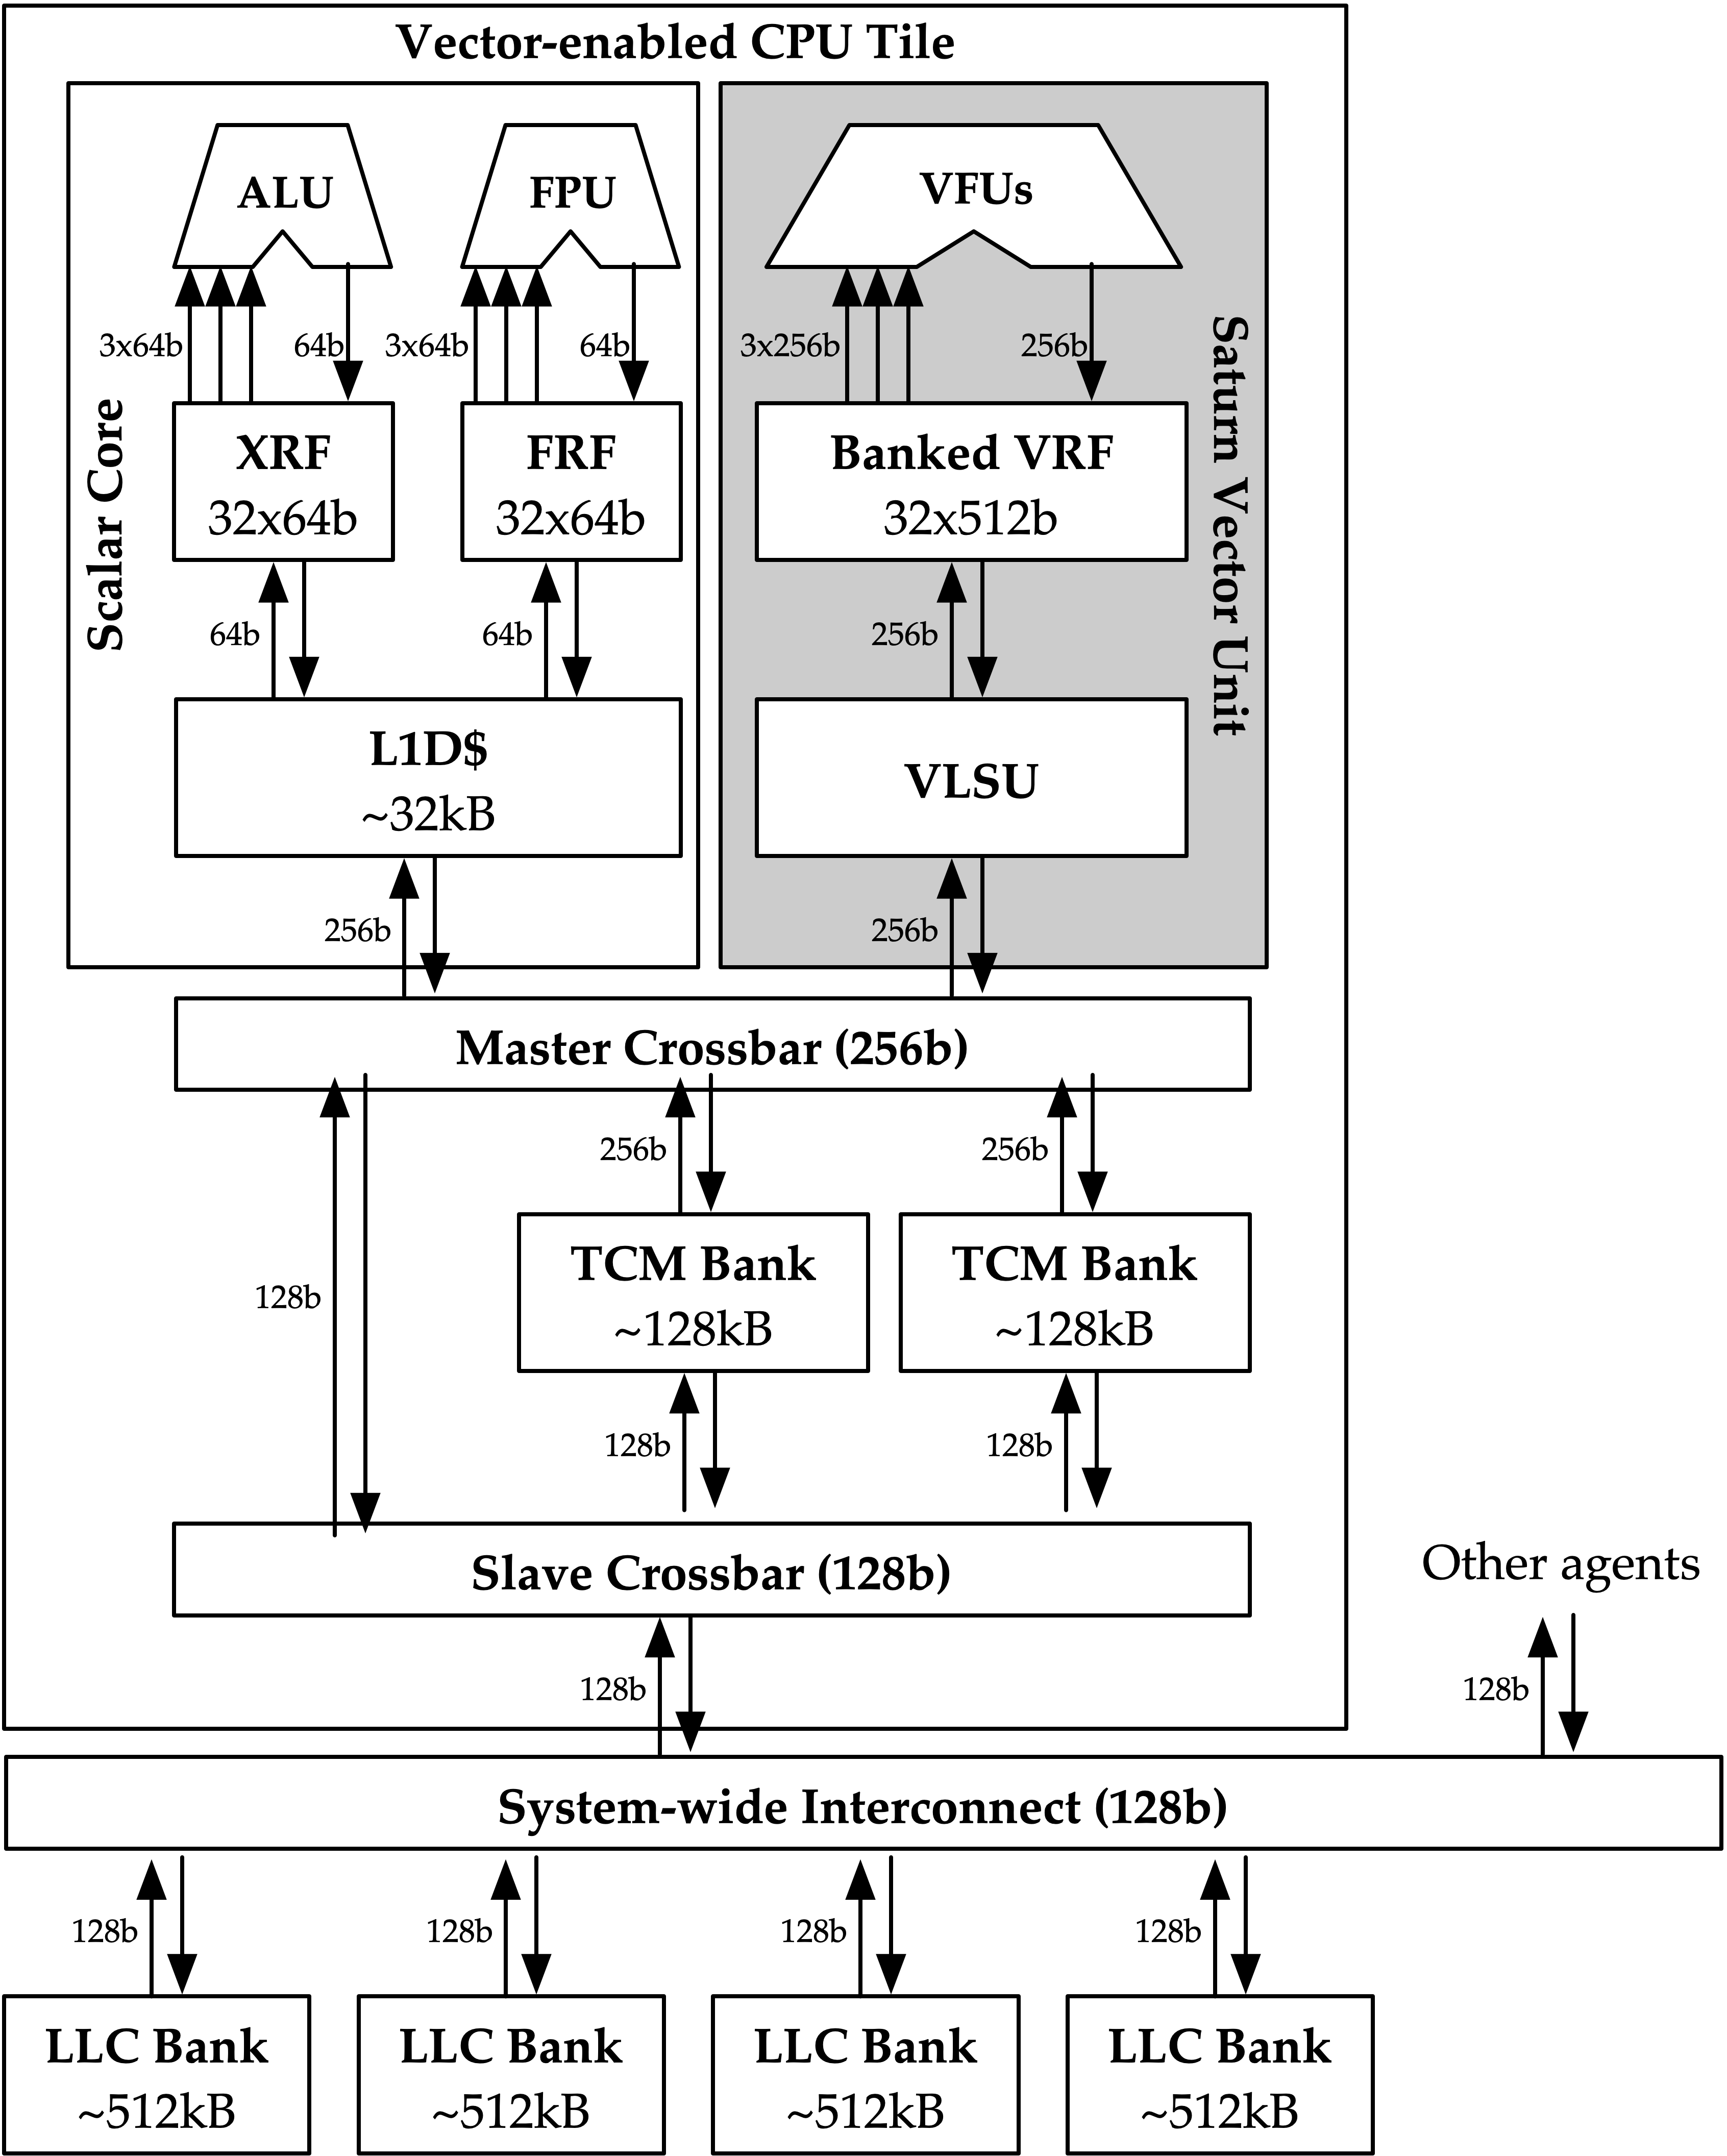
\includegraphics[scale=0.5]{memtcm.png}
  \caption{Example Saturn memory system with high-bandwidth local TCM (Tightly-coupled memory)}
  \label{fig:mem-tcm}
\end{figure}

Saturn configurations with high \texttt{DLEN} would generally require higher memory bandwidth.
However, scaling up the system-level interconnect to meet Saturn's bandwidth demands may be prohibitively costly.
Instead, the preferred approach for high-\texttt{DLEN} Saturn configs is to integrate a high-bandwidth local TCM (tightly-coupled memory), which software should treat as a software-managed cache for vector accesses.
This TCM should be tile-local and globally addressable, but not necessarily cacheable.
Figure \ref{fig:mem-tcm} depicts a Saturn configuration with a high-bandwidth TCM, but a reduced-bandwidth system interconnect.

Saturn's integration with Shuttle supports these tile-local TCMs.

\begin{figure}[h]
  \centering
  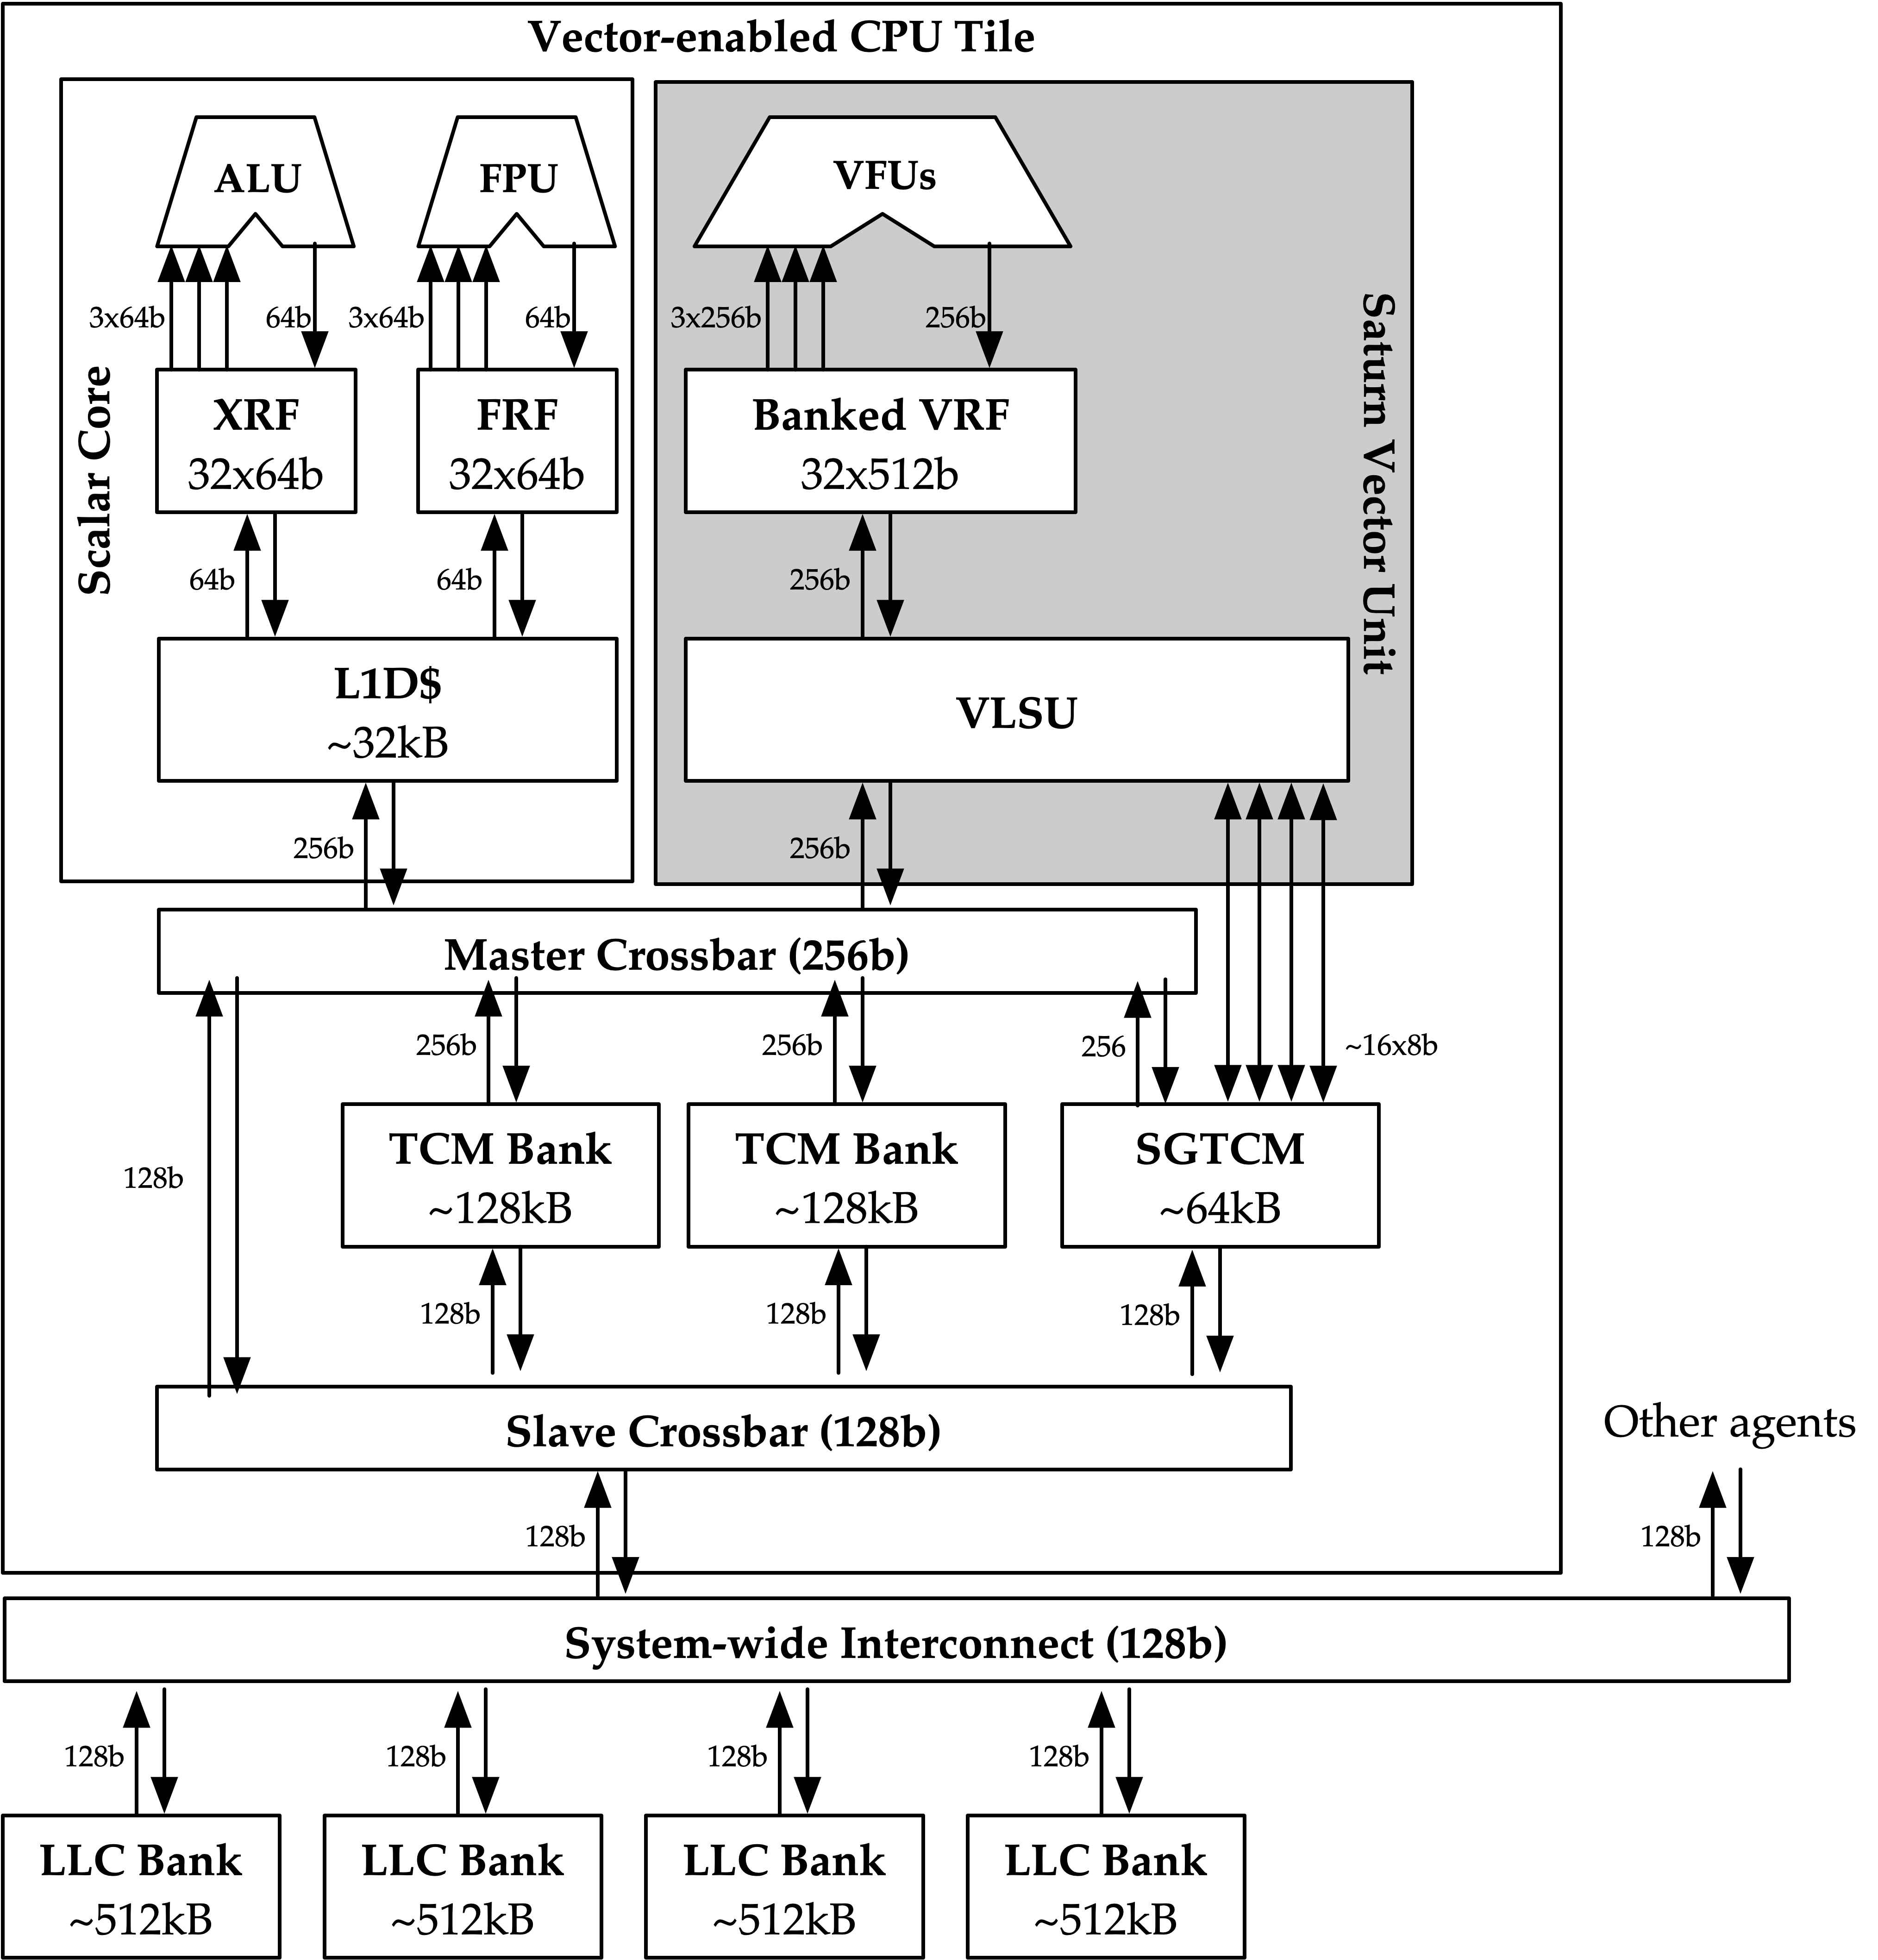
\includegraphics[scale=0.5]{memsgtcm.png}
  \caption{Example Saturn memory system with high-bandwidth local TCM and scatter-gather TCM (SGTCM)}
  \label{fig:mem-sgtcm}
\end{figure}

Saturn also supports integration into a system with a specialized "scatter-gather memory" (SGTCM).
Unlike the standard memory interface, which supports one address per cycle for loads and one address per cycle for stores, the SGTCM interface presents an array of parallel byte-wide ports.
The SGTCM is intended to be implemented as a specialized non-cacheable core-local memory.

Figure \ref{fig:mem-sgtcm} depicts how the Saturn VLSU can be parameterized to bypass the block memory port to access a specialized address-generation engine for a deeply-banked scatter-gather memory.
Saturn's integration with Shuttle supports a byte-wise banked SGTCM.

\subsection{Inflight Instruction Queues}
Upon dispatch from the VFU into the VLSU, a vector memory instruction is written into either the load instruction queue (VLIQ) or store instruction queue (VSIQ).

Each entry in this queue contains the base offset, physical page index, and stride, as well as a bit-mask of older vector loads or stores.
The VFU guarantees that all instructions dispatched into the VLSU have been cracked into operations with single-page access extents.
As a result, the base offset and stride are stored as 12 bits of page offset, while a physical page index provides the upper bits of the address.
Each entry additionally contains the \texttt{vstart}, \texttt{vl}, \texttt{segstart}, and \texttt{segend} settings of this instruction, along with all the fields for addressing mode, element width, index width, and mask control.

The entry also contains a bound (extent) for the instruction's memory access within its accessed page.
This is derived from the base offset, stride, \texttt{vl}, and addressing mode settings of the instruction, but is encoded directly within the entry to enable fast disambiguation checks.
Instructions with indexed accesses are marked conservatively as accessing the entire page.

Memory disambiguation checks are performed using a CAM-like structure over all the entries in the VLIQ or VSIQ to find the entries accessing the same page.
The base and extent of a given access can be checked against the base and extent of the access in the entry to determine if overlap exists.
Both vector-vector and vector-scalar ordering checks use this CAM.

The address sequencer and segment buffer units derive their control signals from pointers into the inflight instruction queues.
For long-chime instructions (when \texttt{LMUL} is high), these pointers can reference the same instruction, enabling a single instruction to occupy all the units in the load or store path.
For short-chime instructions (when \texttt{LMUL} is low), these pointers can refer to different instructions, enabling many simultaneous inflight instructions for short-chime code in a high-latency memory system.

\subsection{Vector-Vector Memory Disambiguation}
\label{sec:vector-disambig}

Saturn is responsible for stalling vector or scalar requests if an older vector or scalar request has not been made visible to the coherent memory system, and would cause a violation of the memory model if the younger request was allowed to proceed.

\begin{itemize}
\item A younger scalar load must stall until all older vector stores to the same address have been issued and acknowledged.
\item A younger scalar store must stall until all older vector loads to the same address have been completed and all older vector stores to the same address have been issued and acknowledged
\item A vector load or store cannot begin execution while there are pending older scalar stores in the scalar store buffer
\item A younger vector load cannot issue requests while there are pending older vector stores to the same address
\item A younger vector store cannot issue requests while there are pending older vector loads to the same address
\end{itemize}

Section \ref{sec:scalar-disambig} discusses how scalar-vector memory disambiguation is managed, while this section discusses the vector-vector cases.
Vector memory disambiguation is performed when instructions enter either the LAS or SAS. An instruction cannot sequence address generation operations through either address sequencer until it has cross-checked the appropriate sequencer for older instructions with overlapping access extents.

The cross-check compares the to-be-address-sequenced instruction's extent with the extent of older instructions in the relevant inflight queue with a CAM-like structure.
Since the VLIQ and VSIQ do not need to be deep, as they hold complete vector instructions, this CAM structure has tolerable cost.

Address disambiguation based on the precise extents of vector accesses, as opposed to a coarse cache-line or page-based granularity, requires a more costly CAM-like circuit.
While a static-granularity address CAM can just compare the upper bits of the physical address, determine overlap by precise extents require comparators on the base and bounds of each access, where the width of each comparator is the page offset in Saturn's case.
This costly circuit is necessary to avoid stalls on false-positive conflicts between consecutive contiguous vector loads and stores.

\subsection{Memory Response Ordering}


The VLSU does not assume that the vector memory interface will respond to requests in order.
This further necessitates the implementation of a load-reordering buffer (LROB).
Saturn supports a LROB with as many buffer entries as possible inflight requests.
Saturn additionally supports implementing the LROB with fewer buffer entries than possible inflight requests, for use in scenarios where the outer memory system generally preserves response order, but is not guaranteed to.
In this configuration, the LROB will replay loads when the LROB's buffers overflow, preserving an in-order response stream into the LMU.

The store acknowledgment unit similarly tracks the outstanding store acknowledgments.
Once the final acknowledgment for a given store has arrived, that store can be freed from the VSIQ.

If integrated into a memory system that preserves load response ordering, the LROB can be omitted.
Future improvements to Saturn can add this optimization.

\subsection{Address Sequencing}
The Address Sequencers (LAS/SAS) generate requests for all memory instructions except for indexed accesses into the SGM.
The address sequencers emit requests aligned to the width of the memory interface.
The sequencer can proceed with an instruction once cleared by address disambiguation.

The address sequencers effectively iterate over two nested loops.
The outer loop iterates over the element index while the inner loop iterates over a "segment index" within a segment for segmented accesses.
An index port and mask port provide a stream of indices/masks generated by the VU for indexed and masked operations.

Unit-strided (segmented and non-segmented) accesses do not execute the inner loop, and iterate the outer loop by the number of elements requested by the next request.
These requests saturate the available memory bandwidth.
Masked unit-strided loads ignore the mask settings, instead applying the mask when performing a masked write into the VRF in the VU.
Masked unit-strided stores receive a byte mask from the SMU along with the data bytes, and use this to construct the store request.

Strided and indexed non-segmented accesses do not execute the inner loop, and iterate the outer loop by a single element per cycle.
A mask is generated to select the active bytes within the access for the requested element.
These accesses use the mask port if set by the instruction, and omit generating the request if the element is masked off.

Strided and indexed segmented accesses execute both the outer and inner loop.
The inner loop iterates by the number of elements within a segment available within the next segment, while the outer loop iterates by segment index.
These access the mask port if set by the instruction, and omit generating the request if the segment is masked off.
Generally, these can saturate the memory bandwidth when the size of one segment is larger than the memory width.

The sequencers will stall if the memory interface is not ready or if there are no more tags to track outstanding memory accesses.
When the last request for an instruction has been sent to the memory system, the pointer into the VLIQ/VSIQ for the instruction is incremented, and the next instruction to undergo address sequencing can proceed.

\newpage
\begin{figure}[hbtp]
  \centering
  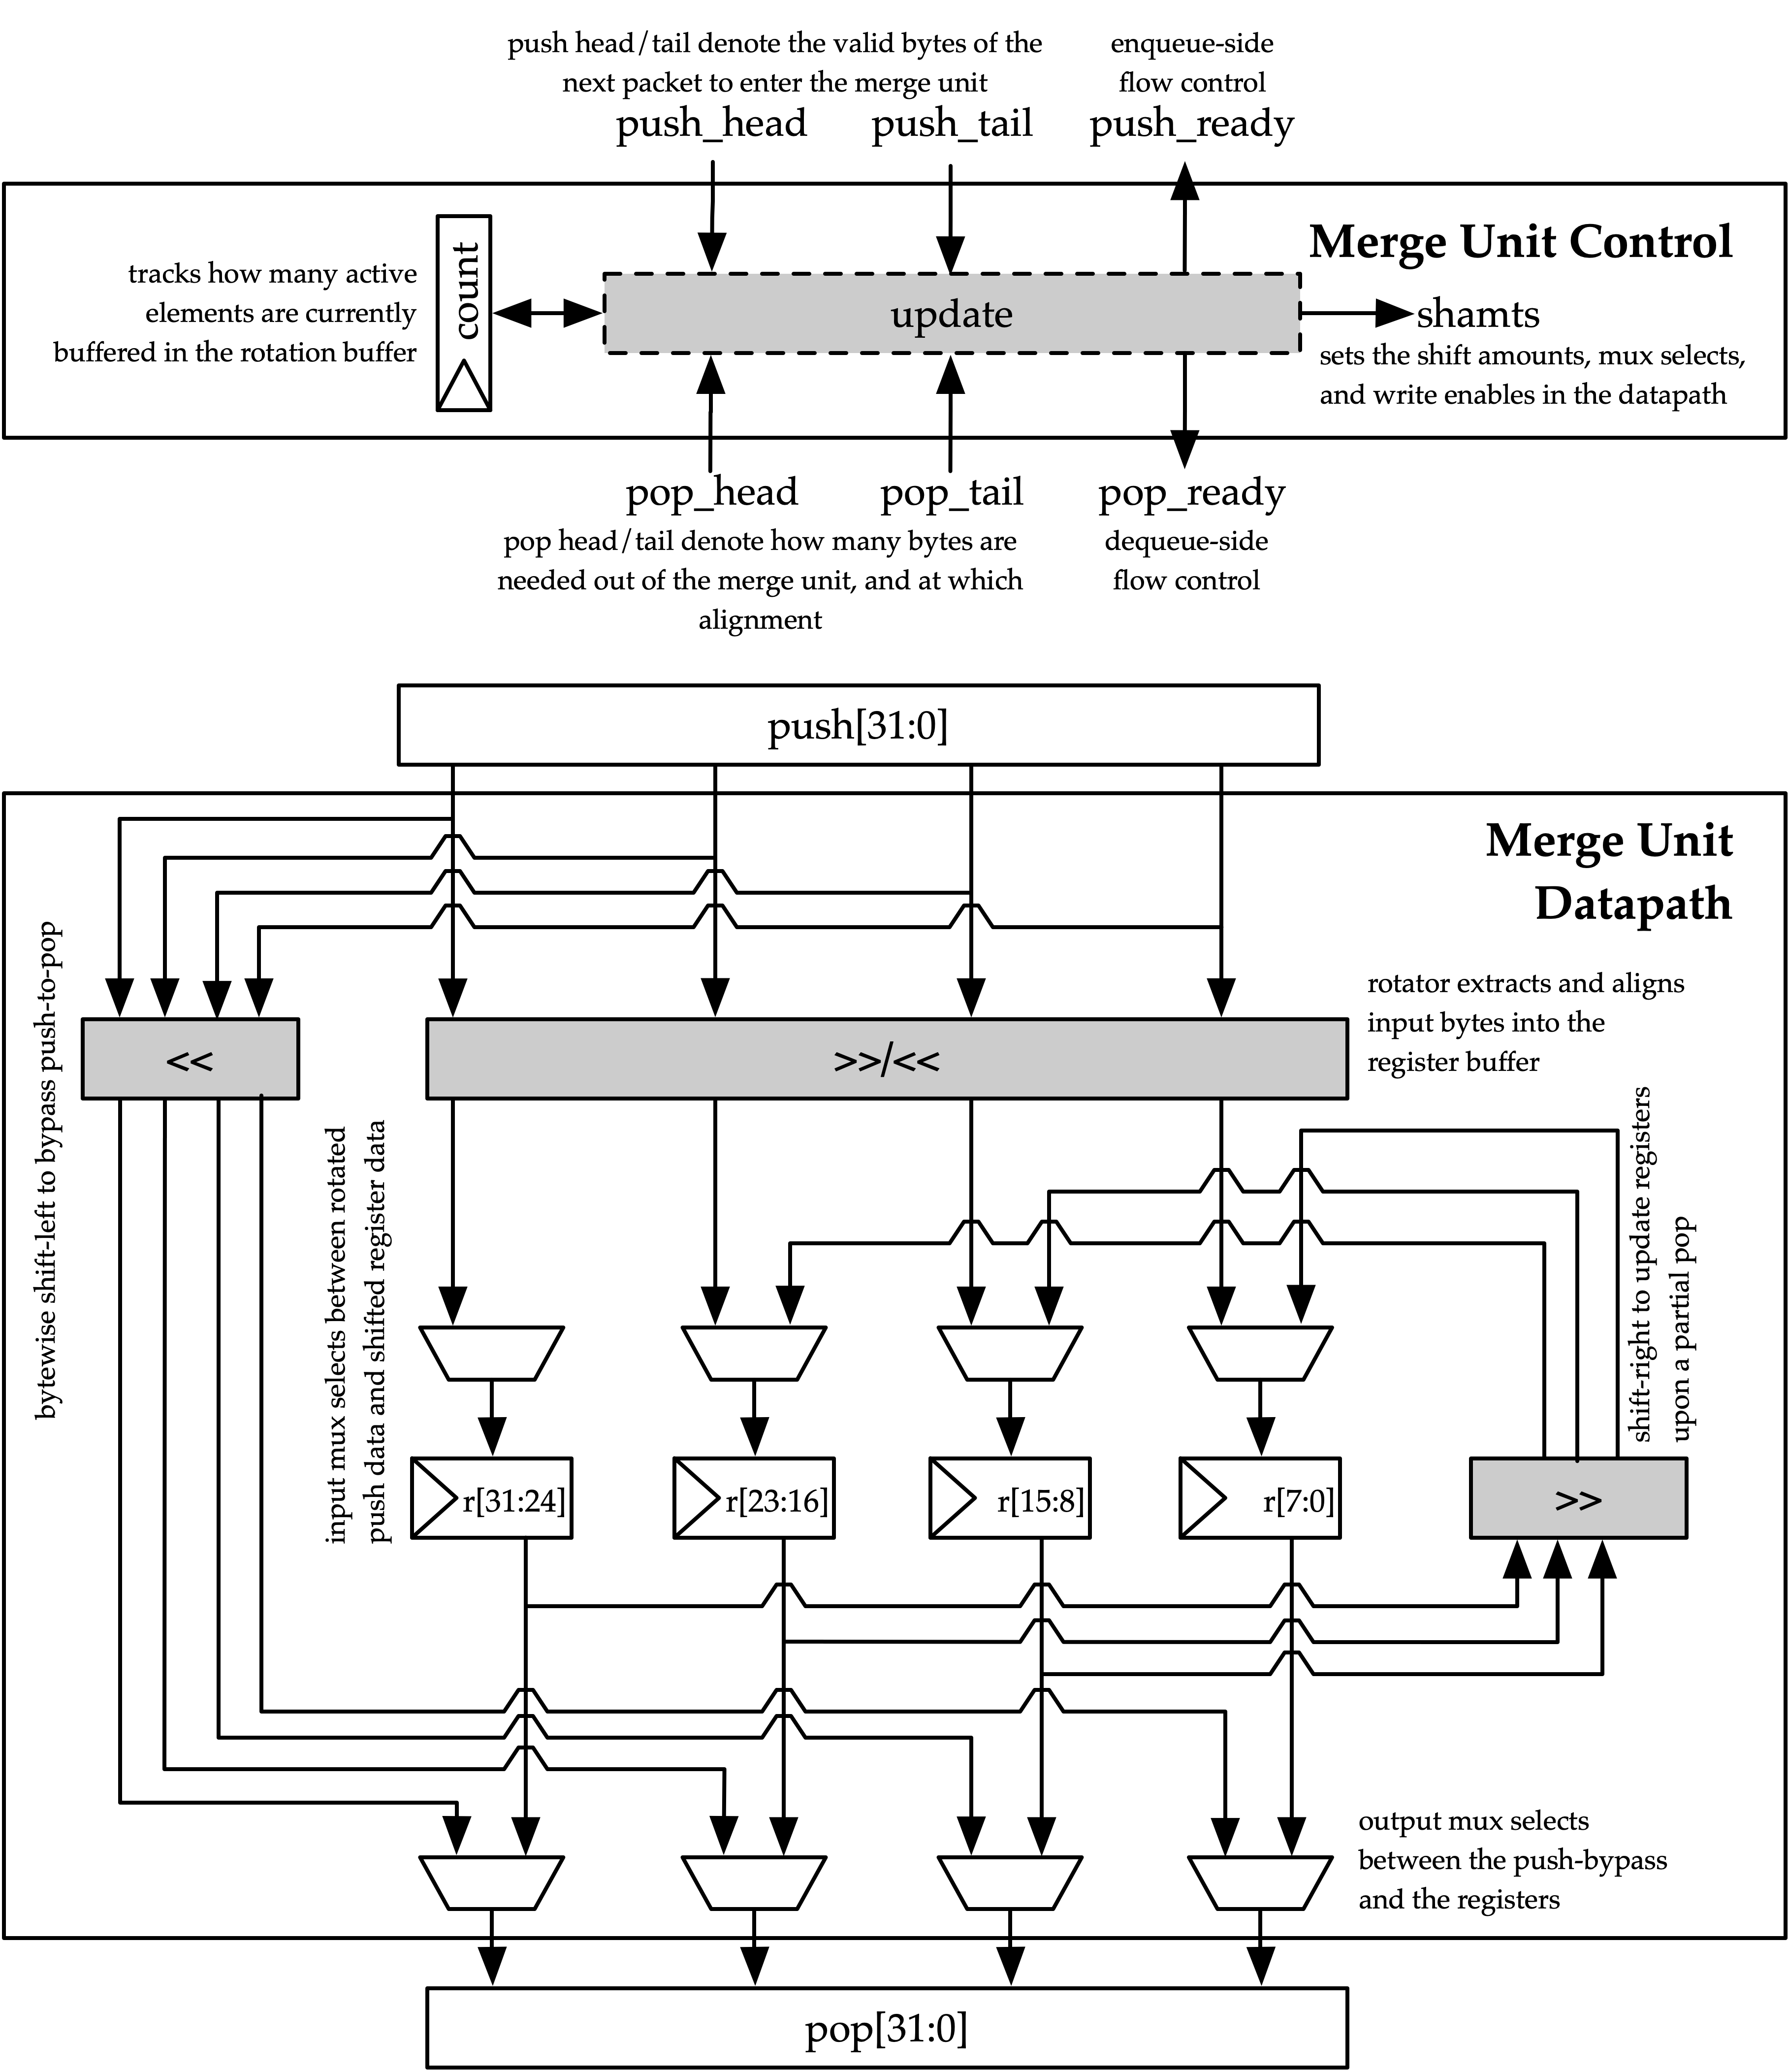
\includegraphics[width=0.8\linewidth]{merger.png}
  \caption{Control and datapath of the merge units. The merge unit can be considered a generalized rotation buffer, where the enqueue and dequeue sides are each latency-insensitive interfaces requesting an update (either a push or pop) of some segment of contiguous valid data into or out of the merge buffer.}
  \label{fig:merge}
\end{figure}

\newpage
\subsection{Merge Units}



The merge units (LMU/SMU) are general-purpose circuits that correct for misalignment of the memory system response data before the next step in the load or store paths.
These can be considered a generalized form of a rotation buffer, decoupling the alignment and extent of input data from the alignment and extent of output data, and preserving latency-insensitive decoupled interfaces.
Microarchitecturally, the merge unit includes two additional byte-shifters compared to a standard rotation buffer.
One additional shifter enables partial dequeues of buffered data, while the other allows the buffer to "compact" many partial packets into a full response packet.

The merge units have FIFO semantics, where the enqueue into the unit specifies a base and extent of active data within the wide input vector.
The merge unit rotates away the inactive bytes, compacting the active bytes into contiguous storage.
The dequeue shifts the buffered data into position based on the requested base and extent.
A bypass path from the enqueue to the dequeue enables full-throughput continuous dataflow for misaligned contiguous accesses.

For the LMU, the push base and extent (head and tail) are set by the address offset associated with the original memory request.
For block-contiguous accesses, only the first and last beat of a single access would encode a non-aligned head or tail, respectively.
For element-indexed or strided accesses where each memory request contains only a single valid element, the push head and tail denote the start and end byte of the active element.
In this way, the LMU serves two roles, either rotating block-contiguous accesses or compressing indexed on strided accesses.
This behavior decouples load-response alignment from writeback; regardless of addressing mode or alignment, the LMU generates aligned \texttt{DLEN}-wide contiguous bytes for writeback in the VU.

For segmented loads, the LMU serves an additional purpose; it enables decoupling of the load write-back scheduling performed by the datapath from the segment restructuring performed by the segment buffer.
That is, the segment buffer does not necessarily proceed at \texttt{DLEN} bits per cycle for all segment sizes.
Depending on the segment size, the segment buffer may request a sub-\texttt{DLEN} slice of bytes, which the LMU will provide once available.

The SMU operates as the reversed path of the LMU.
The push head and tail of the SMU are usually aligned, except for the last element group when \texttt{vl} is misaligned.
For segmented stores, the push head and tail may be set by the store segment buffer, instead of the store datapath.
The pop head and tail are driven by the address alignment generated by the SAS.
Notably, the SMU additionally tracks a byte-wise mask bit for masked stores, such that the mask can be applied to the generated store request.

\subsection{Segment Buffers}

For segmented accesses to proceed with high throughput, the LSB and SSB must "buffer" a sufficient number of responses to "transpose" a set of segments into a set of vector writebacks, or a set of vector store-data into a set of segments.
Non-segmented accesses bypass the segment buffer units entirely.

Each segment buffer is implemented as a double-buffered 2D array of flops.
The double-buffering enables full-rate segmented accesses.
For instance, in the LSB, one half is filled by load responses while the other is drained by load writeback.

Each segment buffer is 8 rows deep to support up to 8 fields in a segment, as required by the specification.
Each segment buffer is \texttt{DLEN} bits wide to buffer entire element groups of writeback data.

Load responses from the LMU write columns into the LSB, while the LSB emits rows into the load writeback port to the VU.
Store data from the VU writes rows into the SSB, while the SSB emits columns into the SMU.

\begin{figure}[hbtp]
  \centering
  \includegraphics[width=\linewidth]{segbuf.png}
  \caption{Table depicting behavior, storage layout, and throughput of the double-buffered LSB for varying NF/ELEN on a DLEN=64b configuration.}
  \label{fig:segbuf}
\end{figure}

Figure \ref{fig:segbuf} depicts how the LSB requests aligned segments from the LMU, stores them in a 2D segment buffer array, and presents a stream of aligned write-back data to the datapath.
Notably, some configurations of \texttt{NF} and \texttt{ELEN} result in sub-optimal throughput, underutilizing the memory system.
However, segmented loads and stores will always be more performant than the equivalent sequence of non-segmented loads and stores used in their place.

Some optimizations to improve the throughput of the power-of-two \texttt{NF} instructions have yet-to-be implemented.
